\documentclass{standalone}
\usepackage{graphicx}
\usepackage{tikz}
\usetikzlibrary{shapes.geometric, arrows, positioning}

\begin{document}

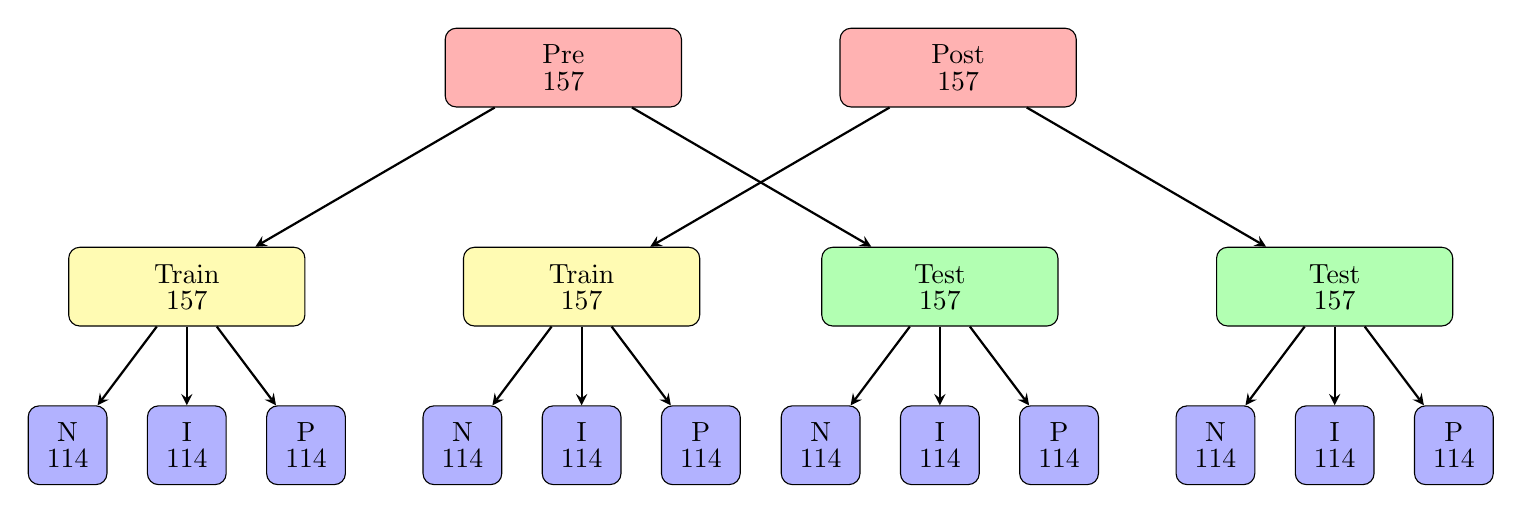
\begin{tikzpicture}[node distance=2cm]
% How to define a shape with specific name
\tikzstyle{red_box} = [rectangle, rounded corners, minimum width=3cm, minimum height=1cm,text centered, draw=black, fill=red!30]
\tikzstyle{yellow_box} = [rectangle, rounded corners, minimum width=3cm, minimum height=1cm,text centered, draw=black, fill=yellow!30]
\tikzstyle{green_box} = [rectangle, rounded corners, minimum width=3cm, minimum height=1cm,text centered, draw=black, fill=green!30]
\tikzstyle{blue_box} = [rectangle, rounded corners, minimum width=1cm, minimum height=1cm,text centered, draw=black, fill=blue!30]
\tikzstyle{arrow} = [thick,->,>=stealth]
% Start initiating nodes
\node (pre) [red_box] {{\shortstack{Pre\\157}}};
\node (post) [red_box, right=of pre] {{\shortstack{Post\\157}}};
\node (pre_train) [yellow_box, below left= 2.5cm of pre] {{\shortstack{Train\\157}}};
\node (pre_test) [green_box, below right= 2.5cm of pre] {{\shortstack{Test\\157}}};
\node (post_train) [yellow_box, below left= 2.5cm of post] {{\shortstack{Train\\157}}};
\node (post_test) [green_box, below right= 2.5cm of post] {{\shortstack{Test\\157}}};

\node (i_pre_train) [blue_box, below =1cm of pre_train] { {\shortstack{I\\114}}};
\node (n_pre_train) [blue_box,  left=0.5cm of i_pre_train] { {\shortstack{N\\114}}};
\node (p_pre_train) [blue_box, right=0.5cm of i_pre_train] { {\shortstack{P\\114}}};

\node (i_pre_test) [blue_box, below =1cm of pre_test] { {\shortstack{I\\114}}};
\node (n_pre_test) [blue_box,  left=0.5cm of i_pre_test] { {\shortstack{N\\114}}};
\node (p_pre_test) [blue_box, right=0.5cm of i_pre_test] { {\shortstack{P\\114}}};

\node (i_post_train) [blue_box, below =1cm of post_train] { {\shortstack{I\\114}}};
\node (n_post_train) [blue_box,  left=0.5cm of i_post_train] { {\shortstack{N\\114}}};
\node (p_post_train) [blue_box, right=0.5cm of i_post_train] { {\shortstack{P\\114}}};

\node (i_post_test) [blue_box, below =1cm of post_test] { {\shortstack{I\\114}}};
\node (n_post_test) [blue_box,  left=0.5cm of i_post_test] { {\shortstack{N\\114}}};
\node (p_post_test) [blue_box, right=0.5cm of i_post_test] { {\shortstack{P\\114}}};

% Draw arrows for connection
\draw [arrow] (pre) -- (pre_train);
\draw [arrow] (pre) -- (pre_test);
\draw [arrow] (post) -- (post_train);
\draw [arrow] (post) -- (post_test);

\draw [arrow] (pre_train) -- (n_pre_train);
\draw [arrow] (pre_train) -- (i_pre_train);
\draw [arrow] (pre_train) -- (p_pre_train);

\draw [arrow] (pre_test) -- (n_pre_test);
\draw [arrow] (pre_test) -- (i_pre_test);
\draw [arrow] (pre_test) -- (p_pre_test);

\draw [arrow] (post_train) -- (n_post_train);
\draw [arrow] (post_train) -- (i_post_train);
\draw [arrow] (post_train) -- (p_post_train);

\draw [arrow] (post_test) -- (n_post_test);
\draw [arrow] (post_test) -- (i_post_test);
\draw [arrow] (post_test) -- (p_post_test);
\end{tikzpicture}

\end{document}